%%% Learning the haptic characteristics of objects by exploration in-hand

\paragraph{(a) Definition of control strategies for concurrent stable object grasping and object surface tracing for haptic exploration}

An Arimoto-PD regulator provides the required torques to track a reference position. The position control law is
\begin{equation}
    \bm{\tau_p} = G(\bm{q}) + K_{P_p} \left(\bm{\dot{q}_d}\Delta T\right) + K_{D_p}\bm{\dot{q}},
\end{equation}
where $G(\bm{q})$ is the gravity load vector, $\bm{{q}}$  is the generalized joint variables, $\bm{\dot{q}}$ is the measured rate of joints variables, $\Delta T$ the control period, and $K_{P_p}$,$K_{D_p}$ two positive definite matrices.

% \begin{figure}
% \begin{center}
% 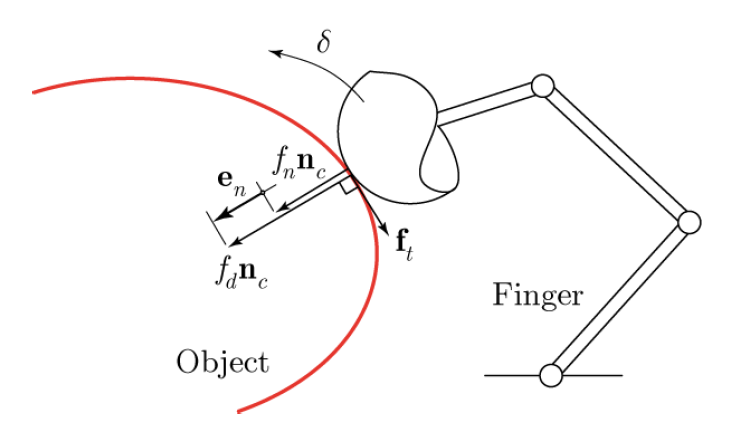
\includegraphics[width=0.65\textwidth]{finger_surface.png}
% \caption{Finger in contact with the unknown surface}
% \label{fig:finger_surface}
% \end{center}
% \end{figure}

A PID force controller is required to ensure contact during motion. The force control law is
\begin{equation}
    \bm{\tau_f} = f_dJ^T\bm{n_c} + K_{P_f}\bm{\tau_{e_n}} + K_{I_f}\int\bm{\tau_{e_n}}dt + K_{D_f}\dot{\bm{\tau}}_{e_n},
\end{equation}
where $J$ is the robot Jacobian matrix, $\bm{e_n} = (f_d - f_n)\bm{n_c}$ is the normal force error, $\bm{\tau_{e_n}} = J^T(\bm{q})\bm{e_n}$ is the normal force error in terms of joints torques, $\bm{v_d}$ the desired twist of the end effector, and $\bm{\dot{q}_d} = J^+\bm{v_d}$ the desired rate of angular joints.

Note that the position and force are to be controlled on the tangent plane and in the direction normal to it, hence due to their orthogonality, we can decouple the actions and sum up the contribution of each controller to form a hybrid force/position controller.

The strategy to slide a finger over a surface consist in assigning a reference velocity on the tangent plane at the contact point, of the same contact point. Let $C$ be the contact point and $\left\lbrace T \right\rbrace$ the frame with $C$ as origin, such that the $y$-$z$ directions form the local tangent plane and the $x$ direction is normal to the fingertip surface and pointing outwards, the desired twist of the fingertip with respect to $C$ written in $\left\lbrace T \right\rbrace$ is
\begin{equation}
    \bm{^Tv_C}=\left(
    \begin{matrix}
        0\\
        v_{dy}\\
        v_{dz}\\
        0\\
        0\\
        0
    \end{matrix}\right),
\end{equation}
where $v_{dy}$ and $v_{dz}$ are scalar components of the desired velocity in the local tangent plane, and $\sqrt{{v_{dy}}^2+{v_{dx}}^2}$ the norm of the assigned velocity. This is called the sliding primitive.

The desired twist of the fingertip center point, $P$, written in the end-effector frame $\left\lbrace E \right\rbrace$ is
\begin{equation}
\bm{^Ev_P}=\left(
    \begin{array}{cc}
       \bm{I}_{3x3} & ^E\hat{\bm{c}} \\
       \bm{0}_{3x3} & \bm{I}_{3x3}
    \end{array}
    \right)
    \left(
    \begin{array}{cc}
        R_{ET} & \bm{0}_{3x3} \\
        \bm{0}_{3x3} & R_{ET}
    \end{array}
    \right)
    \bm{{^Tv_C}},
\end{equation}
where $\bm{c}$ is a position vector from the fingertip center to the contact point, and the $\left(\hat{•}\right)$ operator is the skew-symmetric matrix extraction from a vector operator.

The Jacobian relative to the fingertip center is used to obtain the desired joint angle rates as
\begin{equation}
    \bm{\dot{q}_d}=J(\bm{q})\bm{^Ev_P}
\end{equation}

The set-point of the position controller is the updated joint angles
\begin{equation}
    \bm{q_d}=\bm{\dot{q}_d}\Delta_T+\bm{q},
\label{anglejointsreference}
\end{equation}
where $\Delta_T$ is the control period.

%% THE PPC CONTROLLER, NOT SURE TO INCLUDE IT

% A more general class of the adaptive controllers called Prescribed Performance Controller (PPC) proposed by~\cite{DoulgeriPPC} achieves force/position tracking with prescribed performance and ensures no loss of contact with the surface under parametric uncertainties in robot dynamics and contact compliance. Prescribed performance is presented in terms of convergence rate, steady state error and allowed overshoot for the force/position tracking errors.

% The strong limitation of such controller is that it \textbf{is derivated only for a fixed planar surface}; the robustness by utilizing the controller to perform the same task of the Hybrid F/P one is a possible subject of a future work. Altough a complete mathematical derivation of the controller is in ~\cite{DoulgeriPPC}, here the necessary for the implementation is presented.

% Let the base frame be {B}. Let the surface frame be {S} and attached at some point on the surface; its position is denoted by a vector $\bm{p_s} \in R^3$ and its orientation by a matrix $R_s =[\bm{n_s, o_s, a_s}]$, such that $\bm{n_s} \in R^3$ is the unit vector normal to the contact surface pointing inwards.

% Consider also the end effector frame ${\mathcal{E}}$ described by a position vector $\bm{p_t} \in R^3$ and an orientation matrix $R_t$ that can be parameterized by three rotation angles around the axes of the inertia frame, denoted by $\bm{\phi_t} \in R^3$. Let the generalized position be $\bm{p} = [\bm{p_t^T, \phi_t^T}]^T \in R^6$. The generalized velocity $\dot{\bm{p}} = [\dot{\bm{p}}_t^T, \bm{\omega}_t^T]^T$ is related to the joint velocity $\bm{\dot{q}}$ through the robot Jacobian
% \begin{equation}
%   \dot{\bm{p}}=J(\bm{q})\dot{\bm{q}}.
% \end{equation}

% Assume that the position and orientation of the surface is known and hence $\bm{n_s}$ and the generalized normal vector $\bm{n} = [\bm{n^T , 0_3^T}]^T$ can be used to calculate projection matrices $Q_s =[ I_{3 \times 3} - \bm{n_sn_s^T}]$, $Q=[I_{6 \times 6} - \bm{nn^T}]$ to the position/orientation subspace.

% For a planar surface it is possible to derive the material deformation $\chi$ as a function of $\bm{p_s}$ and $\bm{p}$:
% \begin{equation}
%   \chi = r- \bm{n_s^Tp_s+n_s^Tp_t},
% \end{equation}
% and its derivative:
% \begin{equation}
%   \dot{\chi}=\bm{n^T}\dot{\bm{p}}=\bm{n_s^T}\dot{\bm{p_t}},
% \end{equation}
% where a semispherical end effector of radius $r$ is assumed. As the robot interacts with the surface, an interaction wrench $\bm{w} \in R^6$ arises from the contact, that is measured by a force/torque sensor. This force includes both normal $\bm{n}f$ and tangential forces and torques $Q\bm{w}$.

% Assume that the normal force magnitude $f$ is in general a positive monotonically increasing continuously differentiable nonlinear function of the deformation $\chi$, say
% \begin{equation}
% \bar{f}=\begin{cases}
% f(\chi),\, \chi \ge 0\\
% 0,\, \chi <\ 0.
% \end{cases}
% \end{equation}
% We further assume that the \textbf{force deformation relationship} $f(\chi)$ can be modeled by a \textbf{weighted sum of positive powers of the deformation} $\chi$, that is
% \begin{equation}
% f(\chi)=Z_f^T(\chi)\theta_f,
% \end{equation}
% with
% \begin{equation}
% Z_f(\chi)=[\chi^{\mu_1} \ldots \chi^{\mu_{n_f}}], \; \mu_i \in R^+,
% \end{equation}
% and
% \begin{equation}
% \theta_f=[\theta_{f_1} \ldots \theta_{f_2}].
% \end{equation}

% Define also a quantity that will be useful below:

% \begin{equation}
% \vartheta Z_f = \frac{\partial Z_f(\chi)}{\partial \chi}
% \end{equation}

% In a force/position tracking problem the robot end effector is desired to track a force trajectory $\bm{n}f_d(t)$ along the normal to the surface direction and a desired position trajectory $Q_s\bm{p}_{\bm{t}d}(t)$ on the surface. The desired position trajectory $\bm{p}_{\bm{t}d}(t)$ may be defined in local surface coordinates as $\bm{\xi}_{d}(t)=[\xi_{d_1}(t), \xi_{d_2}(t)]^T \in R^2$ and $\bm{p}_{\bm{t}d}(t)$ is then calculated using information on surface position and orientation: $\bm{p}_{\bm{t}d}(t)=R_s[0, \bm{\xi}_{d}^T(t)]^T+\bm{p_s}$. Define also a orientation trajectory $\bm{\phi}_{td}$ an obtain the desired generalized position
% \begin{equation}
%   \bm{p}_d(t)=[\bm{p}_{\bm{t}d}^T(t) \bm{\phi}_{\bm{t}d}^T(t)].
% \end{equation}

% The control objective of PPC is twofold: 1) track the desired generalized position trajectory $Q\bm{p}_d(t)$ on the surface and 2) track the desired force trajectory $\bm{n}f_d(t)$ normal to the surface in presence of parametric uncertainties in the robot dynamics and the force deformation model, while keeping all signals in the closed loop bounded.

% The meaning of prescribed performance is that the position error $\bm{e}_p = Q(\bm{p}-\bm{p}_d)$ and the normal force error $e_f=(f-f_d)$ evolve within a predefined region that is bounded by a decaying function of time. Assuming an error
% signal $e(t)$, ($e(t)$ may be $\bm{e}_p(t)$ or $e_f(t)$), the mathematical expression of prescribed performance is given,
% for $t\ge0$, by the following inequalities
% \begin{equation}
%   \begin{cases}
%       -M\rho(t) <\ e(t) <\ \rho(t),\, e(0) >\ 0\\
%       -\rho(t) <\ e(t) <\ M\rho(t),\, e(0) <\ 0,
%   \end{cases}
% \end{equation}
% with $-1 <\ M <\ 1$ and $\rho(t)$ is a bounded, smooth, strictly positive, decreasing function with $\lim_{t \to \infty}\rho(t)= \rho_\infty >\ 0$. A possible choose for $\rho(t)$ is
% \begin{equation}
%   \rho(t)=(\rho_0-\rho_\infty)\exp(-lt),
% \end{equation}
% with $\rho_0 >\ |e(0)|$, and $\rho_\infty$ representing the maximum permissible size of the tracking error at steady state. The satisfaction of performance bounds for the force error allows us further to guarantee that the robot will never lose the contact with the surface.

% To satisfy both control objectives define the error trasformation
% \begin{equation}
%   \epsilon(t)=T\left(\frac{e(t)}{\rho(t)}\right),
% \end{equation}
% with
% \begin{equation}
% T(x)=\begin{cases}
%   \log\left(\frac{M+x}{1-x}\right),\, e(0) >\ 0\\
%   \log\left(\frac{1+x}{M-x}\right),\, e(0) <\ 0
%   \end{cases}
% \end{equation}

% In this way the satisfaction of the prescribed performance is obtained simply by keeping $\epsilon(t)$ bounded. Thus, let
% \begin{equation}
% \epsilon_f(t)=T_f\left(\frac{e_f(t)}{\rho_f(t)}\right),
% \end{equation}
% \begin{equation}
% {\bm{\epsilon}_p}(t)=\bm{T}_p\left(\frac{{\bm{e}_p}(t)}{{\bm{\rho}_p}(t)}\right),
% \end{equation}
% \begin{equation}
% \vartheta T_f=\frac{\partial T_f}{\partial \left( \frac{e_f}{\rho_f}\right)}\frac{1}{\rho_f},
% \end{equation}
% and
% \begin{equation}
% \vartheta \bm{T}_p=\frac{\partial \bm{T}_p}{\partial \left( \frac{\bm{e}_p}{\bm{\rho}_p}\right)}\frac{1}{\bm{\rho}_p}.
% \end{equation}
% Consider the following reference velocity vector $\dot{\bm{p_r}}$ in the robot tip operational space
% \begin{equation}
%   \dot{\bm{p_r}}=\bm{n}\frac{\dot{f_d}+\frac{\dot{\rho_f}}{\rho_f}\left(Z_f^T\hat{\bm{\theta}}_f-f_d\right)}{\vartheta Z_f^T\hat{\bm{\theta}}_f}+Q\left(\dot{\bm{p_d}}+\frac{\dot{\bm{\rho}_p}}{\bm{\rho}_p}\bm{e}_p\right),
% \end{equation}
% the proposed control law is
% \begin{equation}
%   u=-k_fJ^T\bm{n}\vartheta Z_f^T\hat{\bm{\theta}}_f\vartheta T_f\epsilon_f-k_pJ^TQ\vartheta \bm{T}_p\bm{\epsilon}_p+Z_d^T(\bm{q,\dot{q},\dot{q}_r,\ddot{{q}}_r})\bm{\hat{\theta}}_d+J^T\bm{w}-D\bm{s_q},
% \end{equation}
% where
% \begin{equation}
%   \bm{\dot{q}}_r=J^+\dot{\bm{p_r}}
% \end{equation}
% and
% \begin{equation}
%   \bm{s_q}=\dot{\bm{q}}-\dot{\bm{q_r}}.
% \end{equation}
% Furthermore, we have indicated with $Z_d^T(\bm{q,\dot{q},\dot{q}_r,{\ddot{q}}_r})$ the Slotine Lie regressor of the manipulator. Moreover, $k_f$, $k_p$ are positive scalar control gains and $D$ is a positive definite matrix.

% Note that, $\bm{\hat{\theta}}_f$ and $\bm{\hat{\theta}}_d$ used in the above equations are respectively the estimation of the unknown parameters vectors $\bm{{\theta}}_f$ and $\bm{{\theta}}_d$ provided by the update laws
% \begin{equation}
%   \dot{\bm{\hat{\theta}}}_f=P_f\left\lbrace \Gamma_fk_f\epsilon_f\vartheta T_f\left(\vartheta Z_f\dot{\chi}-\frac{\dot{\rho}_f}{\rho_f}Z_f\right)\right\rbrace
% \end{equation}
% and
% \begin{equation}
%   \dot{\bm{\hat{\theta}}}_d=-\Gamma_dZ_d^T(\bm{q,\dot{q},\dot{q}_r,\ddot{{q}}_r})\bm{s_q},
% \end{equation}
% with $\Gamma_f$ and $\Gamma_d$ positive definite matrices.

\paragraph{(b) Definition of control strategies for concurrent stable object grasping and rolling manipulation to acquire second-order object surface properties}

Based on the previous control framework, rolling over a surface is achieved by defining a reference velocity of the contact point for a pure revolution about an axis laying on the tangent plane and passing through the contact point. Similar to the previous section, the desired twist of the contact point $C$ written with respect to $\left\lbrace T \right\rbrace$ is
\begin{equation}
    \bm{^Tv_C}=\left(
    \begin{array}{c}
        0\\
        0\\
        0\\
        0\\
        \omega_{dy}\\
        \omega_{dz}\\
    \end{array}\right),
\end{equation}
where $\omega_{dy}$ and $\omega_{dz}$ are the scalar components of the desired rolling velocity, and $\sqrt{{\omega_{dy}}^2+{\omega_{dx}}^2}$ is the norm of the assigned velocity. This is called the rolling primitive.

The desired twist of the fingertip center and the desired joint angle rates rate of joint angles are obtained as in the previous paragraph.

To estimate the curvature of the unknown surface, which is a second-order property, it is possible to use Montana's equations for two object in pure rolling contact, namely
\begin{equation}
M_f \dot{\alpha}_f=(K_f+\tilde{K}_0)^{-1}
\left[
\begin{array}{c}
-\omega_y\\
\omega_x\\
\end{array}
\right],
\label{eq:montana}
\end{equation}
where $\dot{\alpha}_f$ is the velocity of the contact point in the local surface chart (measured), $M_f$ is the metric form of the fingertip surface (known), $K_f$ is the curvature form of the fingertip surface (known), $\omega_x$ and $\omega_y$] are the rolling component of the relative angular velocity of the Gauss frame (measured), and $\tilde{K}_0$ is the curvature form of the object surface (estimated).

For a finite rolling motion, it is possible to approximate (\ref{eq:montana}) with
\begin{equation}
M_f \Delta{\alpha}_f=\bar{K}_r
\left[
\begin{array}{c}
-\Delta\theta_y\\
\Delta\theta_x\\
\end{array}
\right],
\label{montanaapprox}
\end{equation}
where
\begin{equation}
\bar{K}_r=(K_f+\tilde{K}_0)^{-1}=
\left(
\begin{array}{cc}
r_1 & r_2 \\
r_2 & r_3
\end{array}
\right),
\end{equation}
or equivalently,
\begin{equation}
    \bm{b}=A\bm{r},
\end{equation}
with
\begin{equation}
    \bm{b}=M_f \Delta{\alpha}_f,
\end{equation}
\begin{equation}
A=\left(
\begin{array}{ccc}
-\Delta\theta_y & \Delta\theta_x & 0\\
0 & -\Delta\theta_y & \Delta\theta_x\\
\end{array}
\right),
\end{equation}
and
\begin{equation}
\bm{r}=\left(
\begin{array}{c}
r_1\\
r_2\\
r_3
\end{array}
\right).
\end{equation}

Therefore, using the generalized inverse as
\begin{equation}
\bm{r}=A^+\bm{b},
\end{equation}
it is possible to estimate the curvature form of the object surface,
\begin{equation}
\tilde{K}_0=\bar{K}_r^{-1}-K_f,
\end{equation}
and by diagonalization,
\begin{equation}
K_0=R^T(\psi)\tilde{K}_0 R(\psi)
\end{equation}
obtain the principal curvature directions given by $\psi$, and principal curvatures at the contact point, $\tilde{K}_0$.

% \section{Quadric model}
% To estimate the unknown surface a quadric model can be assumed:
% \begin{equation}
% S(\bm{r})=\bm{r^TQr+2p^Tr}-k=0
% \end{equation}

% and the normal surface is described by:
% \begin{equation}
% \nabla_r^TS(\bm{c})=2\bm{Qr}+2\bm{p}
% \end{equation}

% where $Q \in R^{3 \times 3}$ and symmetric, $\bm{p} \in R^3$ and $\bm{r} \in R^3$ position vector of the object surface.
% At each contacted point $(c,n_c)$ holds
% \begin{equation}
% \begin{cases}
% S(\bm{c})=0\\
% \nabla_r^TS(\bm{c})+k\bm{n_c}=0
% \end{cases}
% \end{equation}

% From the previuos system of equation holds
% \begin{equation}
% \bm{y=Wa}
% \end{equation}

% with

% \begin{equation}
% \bm{a}=[q_{11}, q_{22}, q_{33}, q_{12}, q_{23}, q_{13}, p_1, p_2, p_3, k]^T
% \end{equation}

% \begin{equation}
% \bm{W}=\left(
% \begin{matrix}
% x^2 & y^2 & z^2 & 2xy & 2yz & 2xz & 2x & 2y & 2z & 0 \\
% x & 0 & 0 & y & 0 & z & 1 & 0 & 0 & n_x\\
% 0 & y & 0 & x & z & 0 & 0 & 1 & 0 & n_y\\
% 0 & 0 & z & 0 & y & x & 0 & 0 & 1 & n_z
% \end{matrix}
% \right)
% \end{equation}

% \begin{equation}
% \bm{y}=[1,0,0,0]^T
% \end{equation}

% The estimation can be made in batch processing. After N contact points have been registered, solve:

% \begin{equation}
% \bm{a}=\bar{\bm{W}}^+\bar{\bm{y}}
% \end{equation}

% with $\bar{\bm{W}} \in R^{4N \times 10}$ and $\bar{\bm{y}} \in R^{4N}$

\paragraph{(c) Definition of strategies for frictional coefficient estimation}
Using the strategy described in paragraph (a), one can compensate for the tangential force generated due to the frictional property of the object. The tangential force can be extracted from the measured contact force as
\begin{equation}
    \mathbf{f}_t = (I-\mathbf{n}_{c}\mathbf{n}^T_{c})\mathbf{f}_c,
\end{equation}
and the dynamic friction coefficient at the contact point can be readily obtained as
\begin{equation}
    \mu_{d} = \lVert{\mathbf{f}_{t}}\rVert/\lVert{\mathbf{f}_{n}}\rVert.
\end{equation}

Knowing the fingertip material and using a typical look-up table for friction coefficients, one can query by the pair material-dynamic coefficient, and thus obtain the static coefficient, as a well as the object material.

Finally, the compensation will be achieved by adding the term
\begin{equation}
    \boldsymbol{\tau}_f=-J^T \mathbf{f}_t,
\end{equation}
to the force controller.

\paragraph{(d) Testing in simulation}
The simulation framework is heavily based on Adams MSC\copyright, a software for multi-body dynamic simulation and collision management. It uses several contact models based on a penalty formulation on the inter-penetration between meshes. The geometry engine is responsible for detecting contact between two geometries, locating the points of contact, and calculating the common normal at the contact points. Once the contact kinematics are known, contact forces, which are a function of the contact kinematics, are applied to the intersecting bodies. The model adopted is a Hertzian model, named \emph{Impact} by Adams (see Fig.~\ref{fig:contactedmesh}).

Another feature is the capability to export a Simulink block representing the articulated model with inputs (e.g. joint torques) and outputs (e.g. joint angles, contact wrench). Matlab and Simulink were used to implement the control laws and to manage the results.

Thus, a planar finger with three angular joints was modeled using the parameters in Table~\ref{tab:3R}. The fingertip is a hemisphere of radius $3$ cm.

\begin{table}
\centering
\begin{tabular}{cccccccc}
    \toprule
    \textbf{joint} & $\theta$ & $d$ [m] & $a$ [m] & $\alpha$ & \textbf{Mass [Kg]} & $I_{zz}$ [Kgm] & \textbf{CoG [m]}\\
    \toprule
    1 & $q_1$ & $0$ & $0.05$ & 0 & $0.02$ & $5e^{-6}$ & $(0, -0.0250, 0)^{T}$\\
    \midrule
    2 & $q_2$ & $0$ & $0.05$ & $0$ & $0.02$ & $5e^{-6}$ & $(0, -0.0250, 0)^{T}$\\
    \midrule
    3 & $q_3$ & $0$ & $0.05$ & $0$ & $0.02$ & $5e^{-6}$ & $(0 -0.0250 0)^{T}$\\
    \bottomrule
\end{tabular}
\caption{DH and dynamic parameters of the 3R finger.}
\label{tab:3R}
\end{table}

The controller gains for position and force regulation and contact parameters between the fingertip and the objects were set as in Table~\ref{tab:sim_parameters}. The desired normal component contact force was set to $1$N for all cases.

\begin{figure}
\begin{floatrow}
\ffigbox{%
  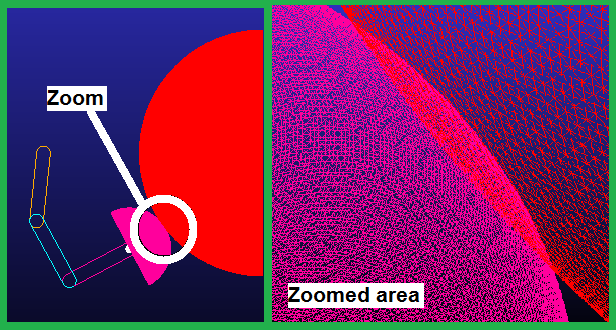
\includegraphics[width=\linewidth]{contacted_mesh.png}%
}{%
\caption{Contact model in Adams.}%
\label{fig:contactedmesh}%
}
\capbtabbox{%
    \begin{tabular}{cccc}
    \toprule
    \textbf{Parameter} & \textbf{Value}\\
    \toprule
    $K_{P_p};K_{D_p}$ & $100;20$\\
    \midrule
    $K_{P_f};K_{D_f};K_{I_f}$ & $10;1;0.1$\\
    \midrule
    Stiffness & 1000$\frac{N}{m}$\\
    \midrule
    Damping & 20$\frac{Ns}{m}$\\
    \bottomrule
    \end{tabular}
}{%
    \caption{Test parameters.}%
    \label{tab:sim_parameters}%
}
\end{floatrow}
\end{figure}


Fig.~\ref{fig:NormCompContForce} shows the track of the normal component of the contact force for the sliding on a plane and a sphere surface. And Fig.~\ref{fig:TangCompForce} shows the track of the normal and tangential force during rolling over the a plane.

\begin{figure}[!t]
\centering
\mbox{
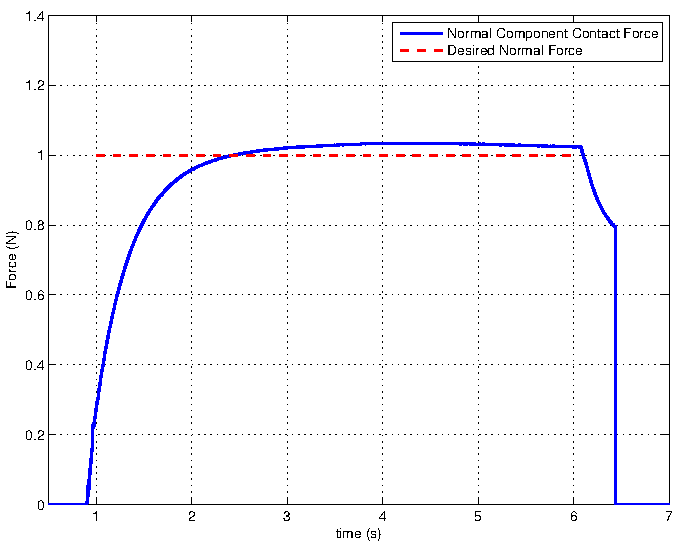
\includegraphics[width=0.45\linewidth]{NormalComponentContactForcePLANE.png}
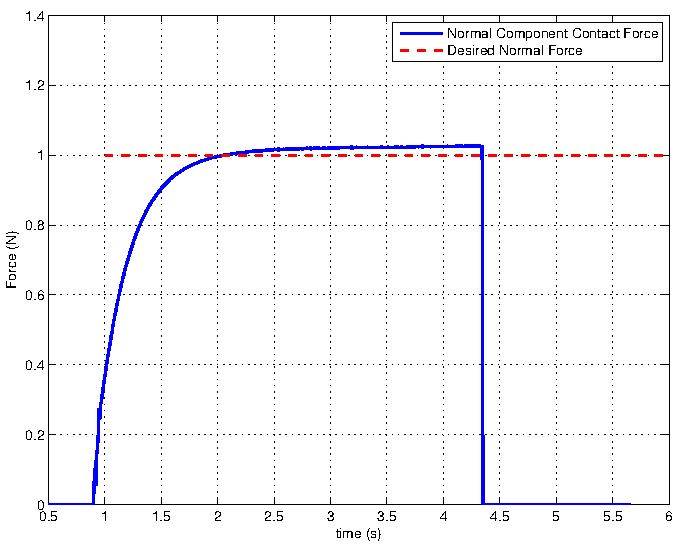
\includegraphics[width=0.45\linewidth]{NormalComponentContactForceSPHERE.png}
}
\caption{Normal component of the contact force when sliding over a plane (left) and a sphere (right).}
\label{fig:NormCompContForce}
\end{figure}

\begin{figure}[!t]
\centering
\mbox{
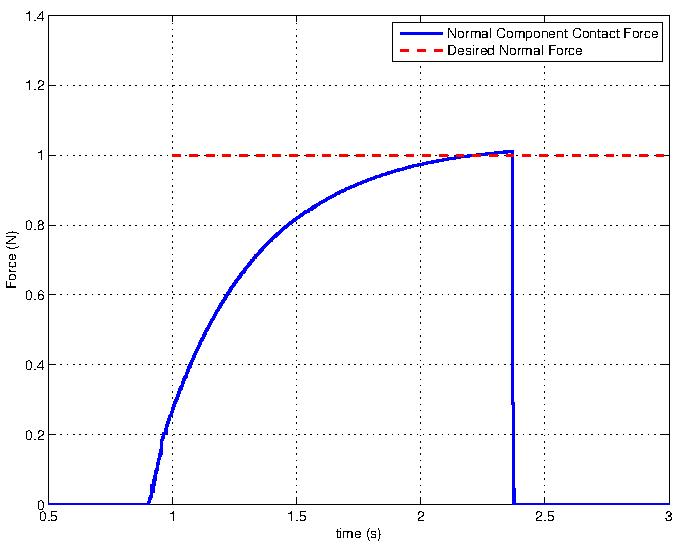
\includegraphics[width=0.45\linewidth]{NormalComponentContactForceROLLPLANE.png}
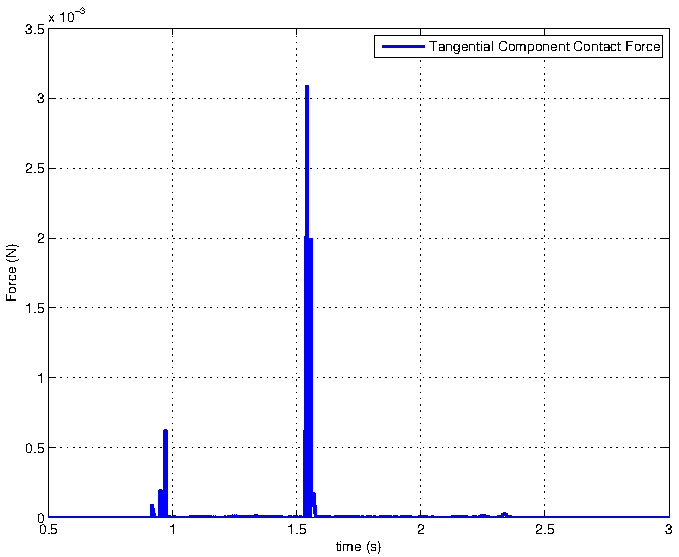
\includegraphics[width=0.45\linewidth]{TangentialComponentContactForceROLLPLANE.png}
}
\caption{Normal (left) and tangential (right) component of the contact force when rolling over a plane.}
\label{fig:TangCompForce}
\end{figure}

The tests were taken to a real scenario shown in Fig.~\ref{fig:curvature}, where the KUKA LWR was equipped with an ATI Nano 17 force torque sensor. The estimated principal curvatures are summarized in Table~\ref{tab:results}. Note that the sphere is a basketball, whose official radius is 11,92-12,07cm, as well as the large values for the plane and one of the principal curvatures on the cylinder.

\begin{table}
\centering
\caption{Experimental Results}
\label{tab:results}
\begin{tabular}{ccccc}
    \toprule
    & \multicolumn{4}{c}{\textbf{Princial Radii}}\\
    \textbf{Object} & \multicolumn{2}{c}{\textbf{Real}} & \multicolumn{2}{c}{\textbf{Estimated}}\\
    \textbf{Direction} & $z$ [m] & $y$ [m] & $z$ [m] & $y$ [m]\\
    \toprule
    Plane & $\infty$ & $\infty$ & 333 & 500 \\
    Cylinder & $\infty$ & .90 & 500 & .088 \\
    Sphere & .1207 & .1207 & 0.121 & 0.127 \\
    \bottomrule
\end{tabular}
\end{table}

\begin{figure}[!h]
    \centering
    \label{fig:curvature}
    \mbox{
    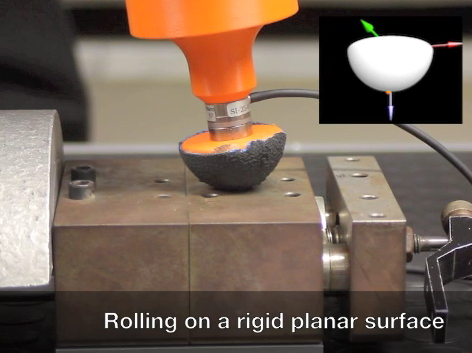
\includegraphics[width=.33\linewidth]{plane}
    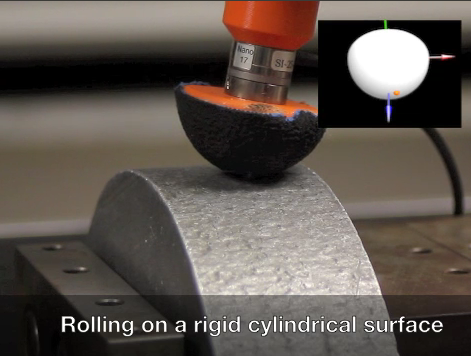
\includegraphics[width=.33\linewidth]{cylinder}
    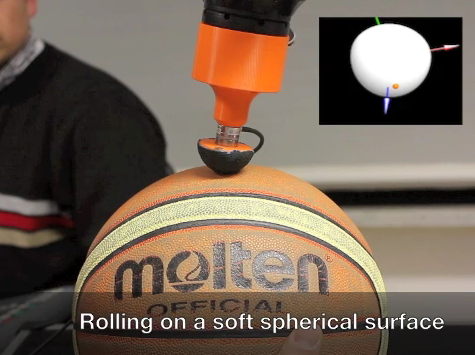
\includegraphics[width=.33\linewidth]{basketball}
    }
    \caption{Test objects for curvature estimation test on a plane (left), a cylinder (middle), and a sphere (right).}
    \vspace{9pt}
\end{figure}


%This results will be tested again in the new simulation framework presented in~\ref{sec:Simulation}.

\paragraph{(e) Integration of object/part model obtained from vision with the code for reactive haptic exploration strategies}

\begin{figure}[!b]
  \begin{center}
    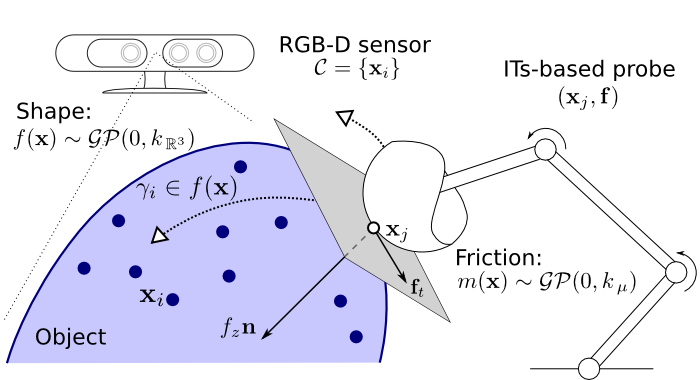
\includegraphics[width=0.8\linewidth]{sliding}
  \end{center}
  \caption{The shape is acquired by an RGBD sensor and the friction coefficients by the intrinsic tactile sensor, both shape~$f(\mathbf{x})$ and friction~$m(\mathbf{x})$ functions are represented as a Gaussian Process $\mathcal{GP}(0,k(\cdot))$. The exploration follows geodesic flows~$\gamma_i$ on the surface of a fixed object using a compliant behavior.}
  \label{fig:schema}
\end{figure}

The setup overview is depicted in Fig.~\ref{fig:schema}. The approach used Gaussian Processes to represent both shape and fiction coefficient. This representation was successfully exploited to generate exploratory trajectories on the object surface, even with arbitrary shapes. The normal contact force was used to distinguish between the contact and the non-contact states. The exploratory probe was the same as in the previous paragraph, with an additional compliant coupler for safety and sensor protection. Only sliding controller was used since the friction coefficient is simpler to retrieve using that primitive. More details on the methodology can be found in Sec.~\ref{sec:slidingPointClouds}.% available at~\href{./attachedPapers/ActiveGatheringOfFrictionalPropertiesFromObjects.pdf}{this link}.

% \begin{figure}[th]
%     \centering
%     \mbox{
%         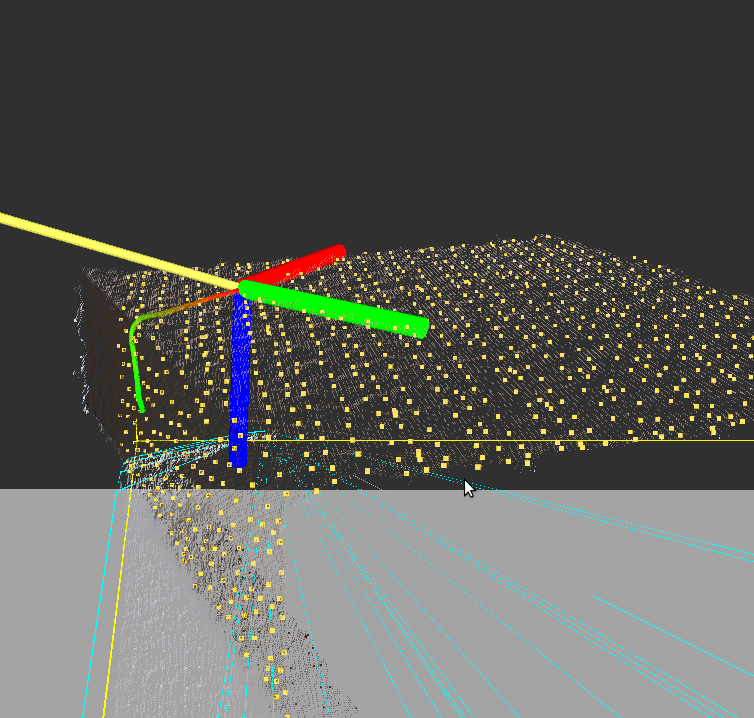
\includegraphics[height=0.4\linewidth]{box.png}
%         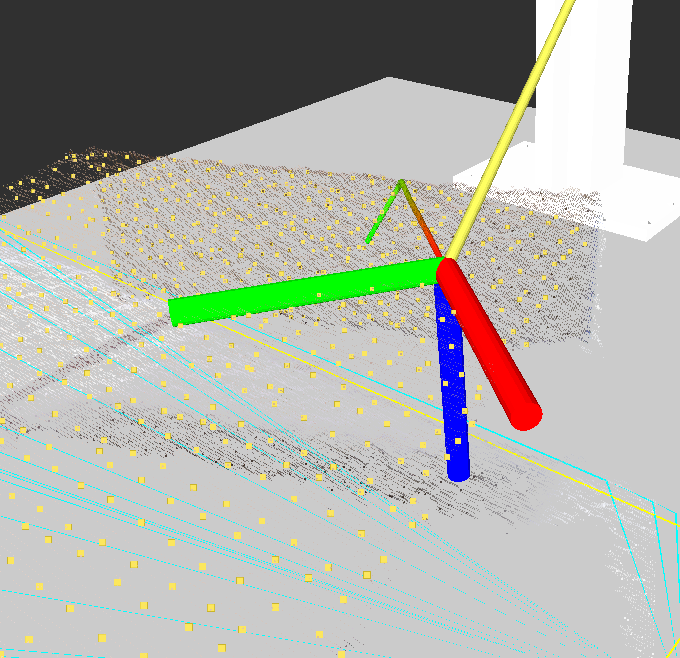
\includegraphics[height=0.4\linewidth]{box1.png}
%         }
%     \mbox{
%         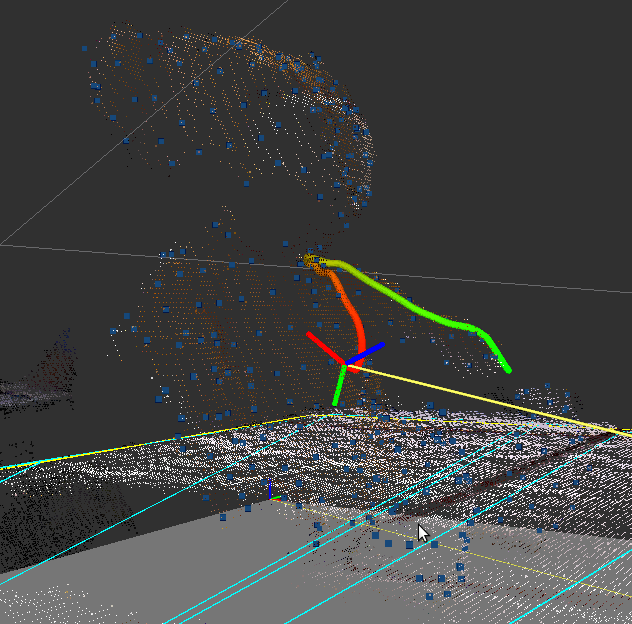
\includegraphics[height=0.4\linewidth]{teddy.png}
%         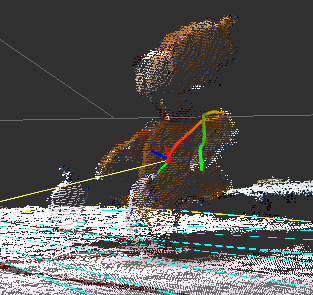
\includegraphics[height=0.4\linewidth]{teddy2.png}
%         }

%     \caption{Geodesic flows on object surfaces captured by an RGBD sensor. The color of the flow goes from red, i.e. the initial contact point, to green, i.e. the final position, according to the predefined length of the curve. The box has flat surfaces, hence geodesics are straight lines (top). The teddy bear has a very irregular shape, but still geodesic flows are found (bottom).}
%     \label{fig:geodesic_examples}
%     \vspace{-0.02\linewidth}
% \end{figure}

% \begin{figure}
%   \centering
%   \mbox{
%         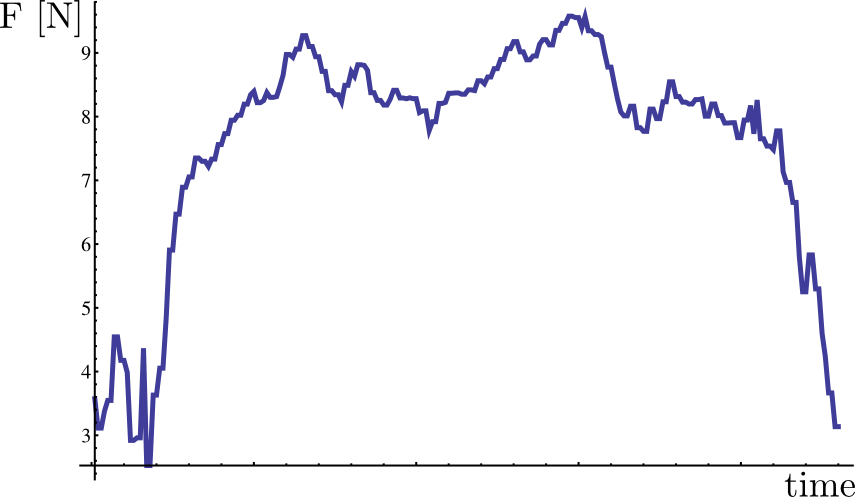
\includegraphics[width=0.45\linewidth]{FZBOX.png}
%         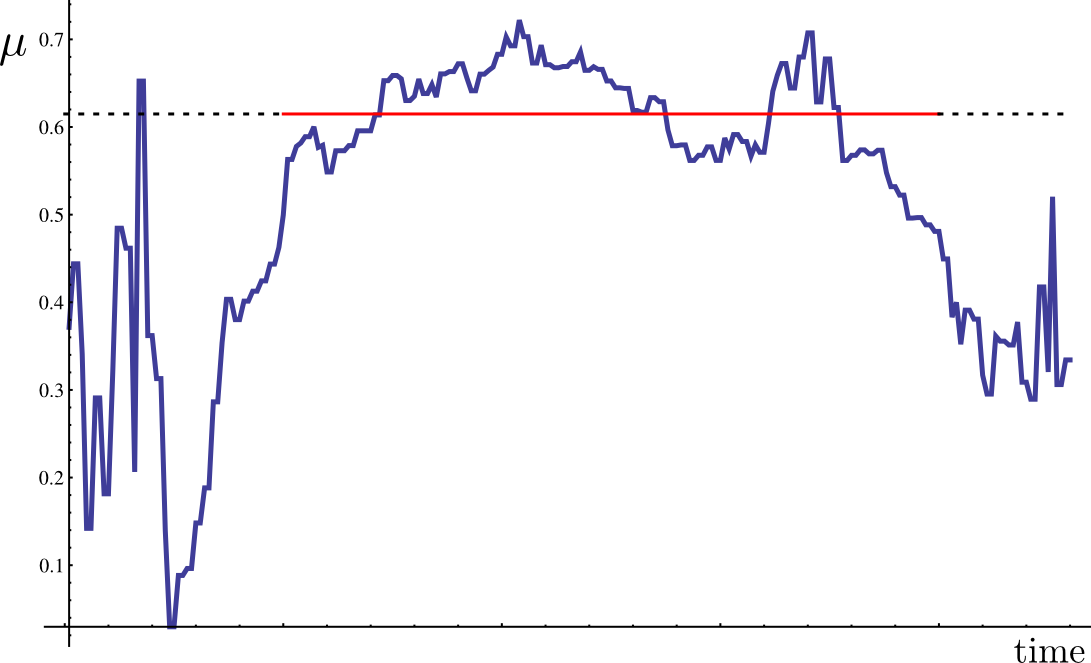
\includegraphics[width=0.45\linewidth]{MuBOX.png}
%         }
%     \caption{Relevant data recorded during a haptic exploration. Force along $\mathbf{z}_{\text{c}}$ used to detect the contact and non-contact states (top). Friction coefficient $\mu$, the red line marks the mean value during the contact state (bottom). Material: Paperboard.}
%     \label{fig:data2}
% \end{figure} 